\documentclass{article}
\usepackage{CJKutf8}
\usepackage[T1]{fontenc}
\usepackage[scaled]{beramono}
\usepackage{graphicx,amsmath,paralist}
\usepackage{epsfig}
\usepackage{subfigure}
\usepackage{color}
\definecolor{bluekeywords}{rgb}{0.13,0.13,1}
\definecolor{greencomments}{rgb}{0,0.5,0}
\definecolor{redstrings}{rgb}{0.9,0,0}

\usepackage{listings}
\lstset{language=C,
showspaces=false,
showtabs=false,
breaklines=true,
showstringspaces=false,
breakatwhitespace=true,
frame=single,
escapeinside={(*@}{@*)},
commentstyle=\color{greencomments},
keywordstyle=\color{bluekeywords}\bfseries,
stringstyle=\color{redstrings},
basicstyle=\ttfamily
}

\usepackage[margin=1.2in]{geometry}

\begin{document}
\begin{CJK}{UTF8}{gbsn}
\title{DSP课程大作业\\
双音多频信号发生和检测}
\author{王亭午,2012011018,无210班\\
杨思怡,2012011010,无210班\\
杨璐馨,2012010995,无210班
}
\date{2015年11月20号}
\maketitle
\section{实验原理}
双音多频DTMF(Dual Tone Multi-Frequency)信令在全世界范围内得到广泛应用,因其提供更高的拨号速率,迅速取代了传统转盘式电话机使用的拨号脉冲信令。近年来DTMF也应用在交互式控制中,诸如语言菜单、语言邮件、电话银行和ATM终端等。将DTMF信令的产生与检测集成到任意一款含有数字信号处理器(DSP)的系统中,是一项较有价值的工程应用。DTMF 编码器在编码时将击键或数字信息转换成双音信号发送出去,解码时在收到的DTMF信号中检测击键或数字信息的存在性。根据CCITT(国际电报电话咨询委员会的简称,它是国际电信联盟(ITU)的常设机构之一) 的建议,国际采用的频率为687Hz、770 Hz 、852 Hz、941 Hz 、1209 Hz、1336 Hz 、1477 Hz和1633Hz等8种。用这8种频率可形成16种不同的组合,从而代表16种不同的数字或功能键。\\
DTMF 用 2 个特定的单音频组合信号代表数字信号,以实现其功能。2 个单音频的频率不同,代表的数字或实现的功能也不同。一个 DTMF 信号由两个频率的音频/波形信号叠加构成。这两个音频信号的频率来自两组预分配的频率组:行频组或列频组(分别对应低频组和高频组)。每一对这样的音频信号唯一表示一个数字或符号。
\subsection{DTMF信号的产生}
在有线电话拨号时,电话机根据当前所拨号码的不同产生不同频率组的电路信号,从而被另一端的交换机所识别,根据每个顺序识别的号码进行预先定义好的线路交换操作。拨号产生的信号即双音多频信号。
\begin{figure}[!h]
\centering
\includegraphics[width=6cm]{dtmf.png}
\caption{DTMF信号的产生}
\end{figure}
双音多频 DTMF(Dual Tone Multi Frequency),由高频群和低频群组成,高低频群各包含4个频率。一个高频信号和一个低频信号叠加组成一个组合信号,代表一个数字。DTMF信号有16个编码。交换机中根据电路的此类双频信号识别用户的播号。DTMF 的具体频率配置如上图所示。\\
DTMF 技术指标要求如下
\begin{compactenum}
\item 采样频率:$8kHz$
\item 传输速率:$10$个数字/秒,或每个数字 $100ms$
\item 信号存在的时间$t$必须满足 $45ms\leq t\leq 55ms,100ms$ 里的其余时间是无声区
\item 高频分量电平不能小于低频分量电平,且电平差不大于 $2dB±1dB$
\item 对于给定的拨号频率,允许的频率偏移为$3\%$
\end{compactenum}
\begin{figure}[h!]
\centering
\includegraphics[width=8cm]{DTMFG.png}
\caption{DTMF信号的产生}
\end{figure}
用 IIR 系统设计数字余弦振荡发生器:
\begin{align*}
y(n)&=-a_1y(n-1)-a_2y(n-2)\\
a_1&=-2cos(\omega_0),a_2=1,\omega_0=2\pi f_0/f_s\\
y(-1)&=0,y(-2)=-A\sin(\omega_0)\\
\end{align*}
其中, $f_s$是采样频率, $f_0$是输出正弦波的频率度,A 为输出正弦波的幅值。装入不同的系数与初始条件(含高、低频组
共两组),就可以一个振荡器对产生所需的八个音频信号,如上图所示。
\subsection{DTMF信号的解调}
对DTMF信号的检测主要是从接收的DTMF信号中恢复出对应的数字信号或功能,需要完成对有效行列频率的检测以及对按键的判决,主要有频谱分析法和带通滤波法:
\subsubsection{频谱分析方法即在频域对DTMF信号进行检测}
完成时域到频域的变换可以用离散傅立叶变换(DFT)或快速傅立叶变换(FFT), FFT计算出所有点的频率,了解信号整个频域信息,而 DFT 可以只计算感兴趣的频率点。如果要计算的频率点数少于 $log_2( N )$,采用 DFT 的计算速度要比 FFT 快一些。如果直接计算 DFT,需要很多复系数,即使只计算一点的 DFT 也需要 N 个复系数。
在我们的实验中,由于只关注DTMF信号的$8$个频率分量的幅度,即我们只关注DFT变换后相应$8$因而我们考虑用 Goertzel 算法,只提取几个频率信号的检测值,明显地提高速度。Goertzel 算法是 DTMF 信号检测的核心。对于 DTMF 信号只用关心其$8$个行频/列频,因此 Goertzel 算法能更快地提取频谱信息。
	\begin{figure}[h!]
	\centering
	\includegraphics[width=8cm]{G.png}
	\caption{DTMF信号的产生}
	\end{figure}
传递函数如下
	\[H_{f_s}(z)=\frac{1-e^{\Omega\pi f_1/f_s}}{1-2\cos\left(\frac{2\pi f_1}{f_s}\right)Z^{-1}+Z^{-2}}\]
对输出信号的计算采用递归方式进行
\[X\left[k\right]=x\left[0\right]+x\left[1\right]W_N+x\left[2\right]W_N^2+\cdots+x\left[N-1\right]W_N^{(N-1)}\]
\[S(n)-W_NS(n-1)=W_N^{-1}\left(S(n-1)-W_NS(n-2)\right)+x(n)\]
\[X(k)=Y(N)=S(N)-W_NS(N-1),W_N=e^{\frac{-2\pi f_1}{f_2}}\]
\[Y(n)=W_N^{-1}Y(n-1)+x(n)\]
\[S(n)=\left(W_N+W_N^{-1}\right)S(n-1)-S(n-2)+x(n)\]
\[S(n)=2\cos\left(\frac{2\pi f_1}{f_s}\right)S(n-1)-S(n-2)+x(n)\]
\[S(-1)=S(-2)=0, n=0,1,\cdots,N\]
如此一来,复杂的复数运算转换成了实数的递归运算,每个频率对应的滤波器只需储存$2\cos\left(\frac{2\pi f_1}{f_s}\right)$一个系数,减小复杂度。
\subsubsection{带通滤波器}
这种方法对接收到的信号进行带通滤波,共有$8$个带通滤波器,分别以$8$个频率为中心频率,这样根据滤波器输出信号的能量情况,便能完成有效行列频的检测及对应按键的判决。带通滤波法的流程如下
	\begin{compactenum}
	\item 根据两组频率值和频率差,确定各带通滤波器的容差指标,并设计带通滤器组
	\item 根据余弦信号的幅度和DTMF信号的信噪比确定各带通滤波器的检测门限
	\item 输入DTMF信号,检测各带通滤波器的输出,利用门限电压来确定DTMF信号的主频,并确定按键数字
	\end{compactenum}
即我们只需要设计滤波器$H_{f_i}(\omega),i=1,2,\cdots,8$, 其中$H_{f_i}(\omega)$为$\left(2\pi f_i -\omega_0,2\pi f_i +\omega_0 \right)$上的带通滤波器,得到经过这几个滤波器后的信号能量,则最高的那两个即为DTMF频率成分。
\section{实验安排}
\subsection{实验难点}
\subsubsection{BF533,BF561系列软硬件接口}
我们的开发板按键的接口如何使用。第一是我们如何把开发板按键变换为我们的输入控制。
第二是:假设我们已经能够产生和处理 DTMF 信号,我们如何接收我们的外部 DTMF 信号?
我们如何发送我们的 DTMF 信号?
\subsubsection{DTMF 信号的产生和处理}
我们可以根据 talkthrough 工程来进行我们项目的修改。但是产生信号和调用信号是我
项目中非常困难的两个部分。
产生信号的时候,我们需要根据我们的按键输入,使用我们的两个二阶数字正弦波振荡器,
我们如何设置我们的输出 SPI 参数呢?
处理信号的时候,我们怎么实现我们的 Goertzel 算法呢?
\subsection{实验分工}
根据我们上面分析的三个主要的实验问题难点,我们的初步分工如下:王亭午负责 DTMF 信号的产生,杨思怡负责 DTMF 信号的处理,杨璐馨同学负责开发板的接口实现。
\subsection{验收方法和指标}
\subsubsection{DTMF信号产生和传输}
以小键盘模拟电话机 16 个按键,完成双音多频信号的发生。即通过小键盘的拨号能够输出对应 DTMF 信号,并可经 DA 输出供测试者听或者交解码器解码。
\subsubsection{DTMF信号处理}
完成双音多频信号的解码,源信号可以来自也可以来自导入的数据文件,也支持来自AD 输入的 DTMF 信号。
\section{实验内容}
\subsection{硬件设置 \textcolor{red}{王亭午部分}}
在实验中,硬件设置主要是值两个地方的设置,一个是我们的按键调用设置,另外一个则是我们的sport设置。
\subsubsection{DMA和SPORT设置}
本次实验中,我们同样采取最为普遍的autobuffering下的sportDA传输。
我们将左右两路声道按照\(I^2S\)协议传输到模拟耳机中去,具体的SPI控制寄存器配置如下:
\begin{lstlisting}
// names for codec registers, used for iCodec1836TxRegs[]
#define DAC_CONTROL_1		0x0000
#define DAC_CONTROL_2		0x1000
#define DAC_VOLUME_0		0x2000
#define DAC_VOLUME_1		0x3000
#define DAC_VOLUME_2		0x4000
#define DAC_VOLUME_3		0x5000
#define DAC_VOLUME_4		0x6000
#define DAC_VOLUME_5		0x7000
#define ADC_0_PEAK_LEVEL	0x8000
#define ADC_1_PEAK_LEVEL	0x9000
#define ADC_2_PEAK_LEVEL	0xA000
#define ADC_3_PEAK_LEVEL	0xB000
#define ADC_CONTROL_1		0xC000
#define ADC_CONTROL_2		0xD000
#define ADC_CONTROL_3		0xE000

// names for slots in ad1836 audio frame
#define INTERNAL_ADC_L0			0
#define INTERNAL_ADC_R0			2
#define INTERNAL_DAC_L0			0
#define INTERNAL_DAC_R0			2
#define INTERNAL_ADC_L1			1
#define INTERNAL_ADC_R1			3
#define INTERNAL_DAC_L1			1
#define INTERNAL_DAC_R1			3
\end{lstlisting}
其中值得注意的是,我们的BF533实际上只支持44.1kHz,32.0kHz,48.0kHz三种格式,因此我们实际上只能对8kHz进行过采样。
这里我们为了方便起见,选用了De-emphasis = 11,也就是使用了48kHz。后面的实验结果证明,因为轮询代码历程本身的低效性,即使是使用32kHz也会出现亚实时的情况出现。因此我们这里不妨就用48kHz。\\
Serial Mode我们选用000,即使用\(I^2S\)协议,Data-Width我们采用16bit的short信号来传输我们的DTMF。综上我们可以得到上面代码中对应的参数。\\
同时,我们也采用了autoBuffering的pingpong技术,缓存的framesize为1024。具体的设置如下:
\begin{lstlisting}
// Configure DMA2
// Ping-Pong Buffer, the first half of TxBuffer is ping, the second half is pong
// 16-bit transfers, 2 dimensional, Autobuffer mode
*pDMA2_CONFIG = WDSIZE_16 | DMA2D | FLOW_1;
// Start address of data buffer
*pDMA2_START_ADDR = (void *)TxBuffer;
// DMA inner loop count
*pDMA2_X_COUNT = 2*FRAMESIZE;
// Inner loop address increment
*pDMA2_X_MODIFY	= 2;
// DMA outer loop count
*pDMA2_Y_COUNT = 2;
// Outer address increment
*pDMA2_Y_MODIFY	= 2;
\end{lstlisting}
注意和talkthrough不同的是,在产生信号阶段我们其实并不需要设置Receive段口。
\subsubsection{按键设置}
这里要注意:\textbf{网络学堂给出的轮询按键代码是有问题的}。在这个地方我们组至少花了3个小时才弄好,感谢一直和我们一起调代码的助教老师!没想到助教老师真的一直和我们一起调,非常感动!下面给出更改的地方:把在243行的下行代码移动到上面的括号中。
\begin{lstlisting}
*pFlashA_PortB_Data = 0x00;
\end{lstlisting}
之前之所以led没有任何反应是因为,上面这一样代码的位置放错之后,每一次轮询之后led灯都被弄回了0的状态。\\
下面进入正题,我们定义并且初始化我们的按键,设置PF管脚的相关寄存器如下:
\begin{lstlisting}
void Init_Flags(void) {
	*pFIO_INEN		= 0x0f00;//
	*pFIO_DIR		= 0x0000;
	*pFIO_EDGE		= 0x0000;//zb:level sensitive
	*pFIO_MASKA_D	= 0x0000;//zb:interruption
}
\end{lstlisting}
在主函数中,我们进行轮询。每次检测到按键被按下,我们就切换到下一个数字。因为DTMF中有16个数字,因此我们进行一个mod(16)的操作。
\begin{lstlisting}
while(1) {
	if((*pFIO_FLAG_D&0x0100)>0) {
		//button SW4 is pressed
		printf("SW4/PF8 pressed down\n");
		if (state == 0) { // the freq changes
			state = 1;
			f = f + 1;
			f = f % 16;
			dtmf(DTMF_Signal, 2 * FRAMESIZE, freq[f][0], freq[f][1], fs, Amp);
		}
	} else { state = 0;
	printf("SW4/PF8 released\n");}
}
\end{lstlisting}
注意,我们需要把对应SW开关的1~6需要置于ON的状态,才能是的对应PF与按键SW相联通。
\subsection{DTMF信号的软件生成 \textcolor{red}{杨璐馨部分}}
\subsubsection{DTMF信号的生成,采样率和过采样率}
DTMF信号的生成中,我们考虑在BF533中生成过采样的49kHz信号。实现代码如下;
\begin{lstlisting}
extern void dtmf(fract16* output, int length2, float f1, float f2, float fs, float Amp) {
	
	int length = length2 / 2;
	
	float a1 = -2 * cos(2 * 3.1415 * f1 / fs);
	float a2 = 1;

	float b1 = -2 * cos(2 * 3.1415 * f2 / fs);
	float b2 = 1;
		
	float out_1[2] = {0, -Amp * sin(2 * 3.1415 * f1 / fs)};  // out_1 is the coeff for f1
	float out_2[2] = {0, -Amp * sin(2 * 3.1415 * f2 / fs)};

	float temp = 0;
	int i = 0;

	for (i = 0; i < length; i ++) {
	    if (i < length / 4 || i > length / 4 * 3) {
			output[i] = 0;
			continue;
		}
		
		temp = - a1 * out_1[0] - a2 * out_1[1];
		out_1[1] = out_1[0];
		out_1[0] = temp;

		temp = - b1 * out_2[0] - b2 * out_2[1];
		out_2[1] = out_2[0];
		out_2[0] = temp;

		output[2 * i] = float_to_fr16((out_1[0] + out_2[0]));
		output[2 * i + 1] = output[2 * i];
	}
	
}
\end{lstlisting}
在上面的代码中,f1,f2是我们对应的双音,fs是我们的实际采样率48kHz。Amp是我们的输出信号幅度。注意到我们的输出16bit short信号的最大值1对应的是我们SPORT输出中的最大值,因此理论上我们只需要保证
\begin{equation}
A_1 + A_2 \leq 1
\end{equation}
就可以保证不发生切顶。不过考虑到初始不稳定值的可能性,我们一般选取\(A_1 = A_2 = 0.4\)。
在上面的式子中,如果我们的信号要采用8000Hz中10个数字,即\(\frac{8000}{10} = 800\)Hz中传输一个数字。
在这个的同时我们需要考虑400个静音的点,那么在\(f_s = 8000\)Hz的情况中,我们只需要令前四分之一和后四分之一的信号为0即可。
\subsubsection{float转化为fract16}
注意到我们产生的信号是float型的,还转换为我们的SPORT需要的型号格式,即short或者fract16格式。
下面是我们根据两个数据的不同格式编写的一个转换函数。
注意到其中0x0f800000是我们用来模拟进位的操作。
\begin{lstlisting}
extern fract16 float_to_fr16(float x) {
	int temp;

	fract32 result;
	temp = *(int *)(&x);

	if ((temp & 0x7f800000) >= 0x3f800000) {
	    result = 0x7fffffff;
	    if (temp < 0)  result = 0x80000000;  // overflow
	} else {
	    temp = temp + 0x0f800000;
	    result = *(float *)(&temp);
	}

	return (result >> 16);
}
\end{lstlisting}
\subsubsection{DTMF信号的传输}
传输的方式很简单,我们在不断的向我们TxPing和TxPong换粗
\begin{lstlisting}
static int ping = 0;
/* core processing in ping-pong mode */
if(0 == ping) {
	memcpy(TxPing, DTMF_Signal, 2*FRAMESIZE*sizeof(RxPing[0]));
} else {
	memcpy(TxPong, DTMF_Signal, 2*FRAMESIZE*sizeof(RxPong[0]));
}
ping ^= 0x1;
\end{lstlisting}
这里的framesize是1024,对应到我们的实际时间是
\begin{equation}
t_0 = 1_s \times 1024 / 48\mbox{kHz}
\end{equation}
因此,上一个section中关于信号静音设置可以更加严谨一些。上面的情况是最为简单的情况,也就是我们的信号没有停顿,不断的发送的情况。
在这个情况下,我们的信号实际上每秒种重复了\(f_s / \mbox{FRAMESIZE}\)次。
如果需要按照信号只产生8000kHz(1秒钟)中的800采样点,然后信号停止,并且信号有400kHz,我们需要在上面的函数中设置计数器。\\
在最后的实验验收中,助教老师已经听到了我们组作出来的电话声。在matlab中最后的结果图如下
\begin{figure}[h!]
\centering
\subfigure[取400Hz静音,频率为1336,770Hz的部分信号]{
\label{Fig.sub.1}
\includegraphics[width=0.45\textwidth]{2_1.eps}}
\subfigure[不取静音,频率为1336,941Hz的部分信号]{
\label{Fig.sub.2}
\includegraphics[width=0.45\textwidth]{1.eps}}
\caption{时域波形片段图}
\label{Fig.lable}
\end{figure}\begin{figure}[h!]
\centering
\subfigure[取400Hz静音,频率为1336,770Hz的频谱信号]{
\label{Fig.2.1}
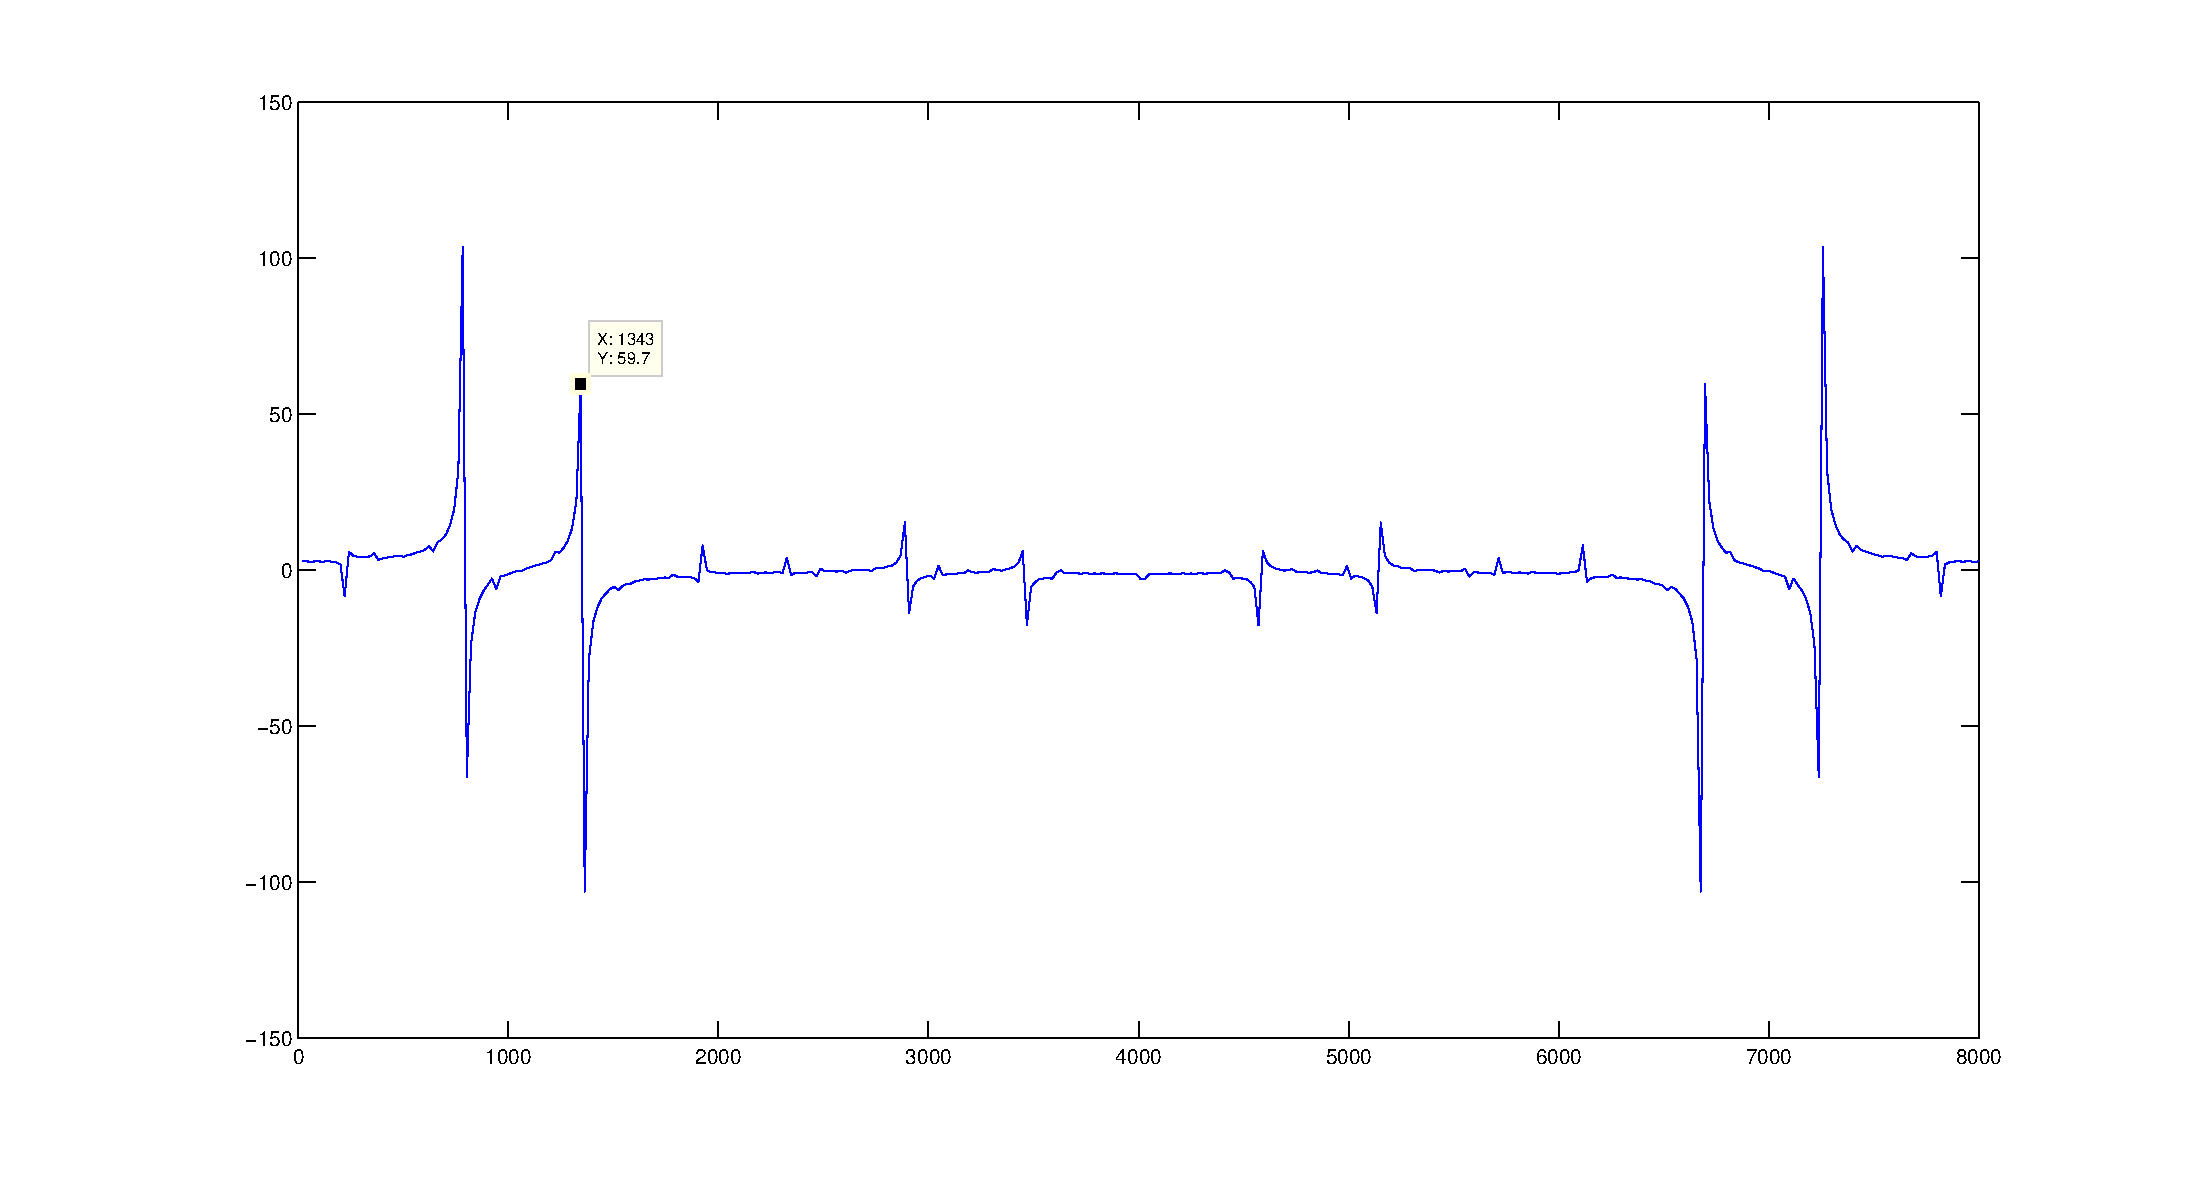
\includegraphics[width=0.45\textwidth]{2_2.eps}}
\subfigure[不取静音,频率为1336,941Hz的频谱信号]{
\label{Fig.2.2}
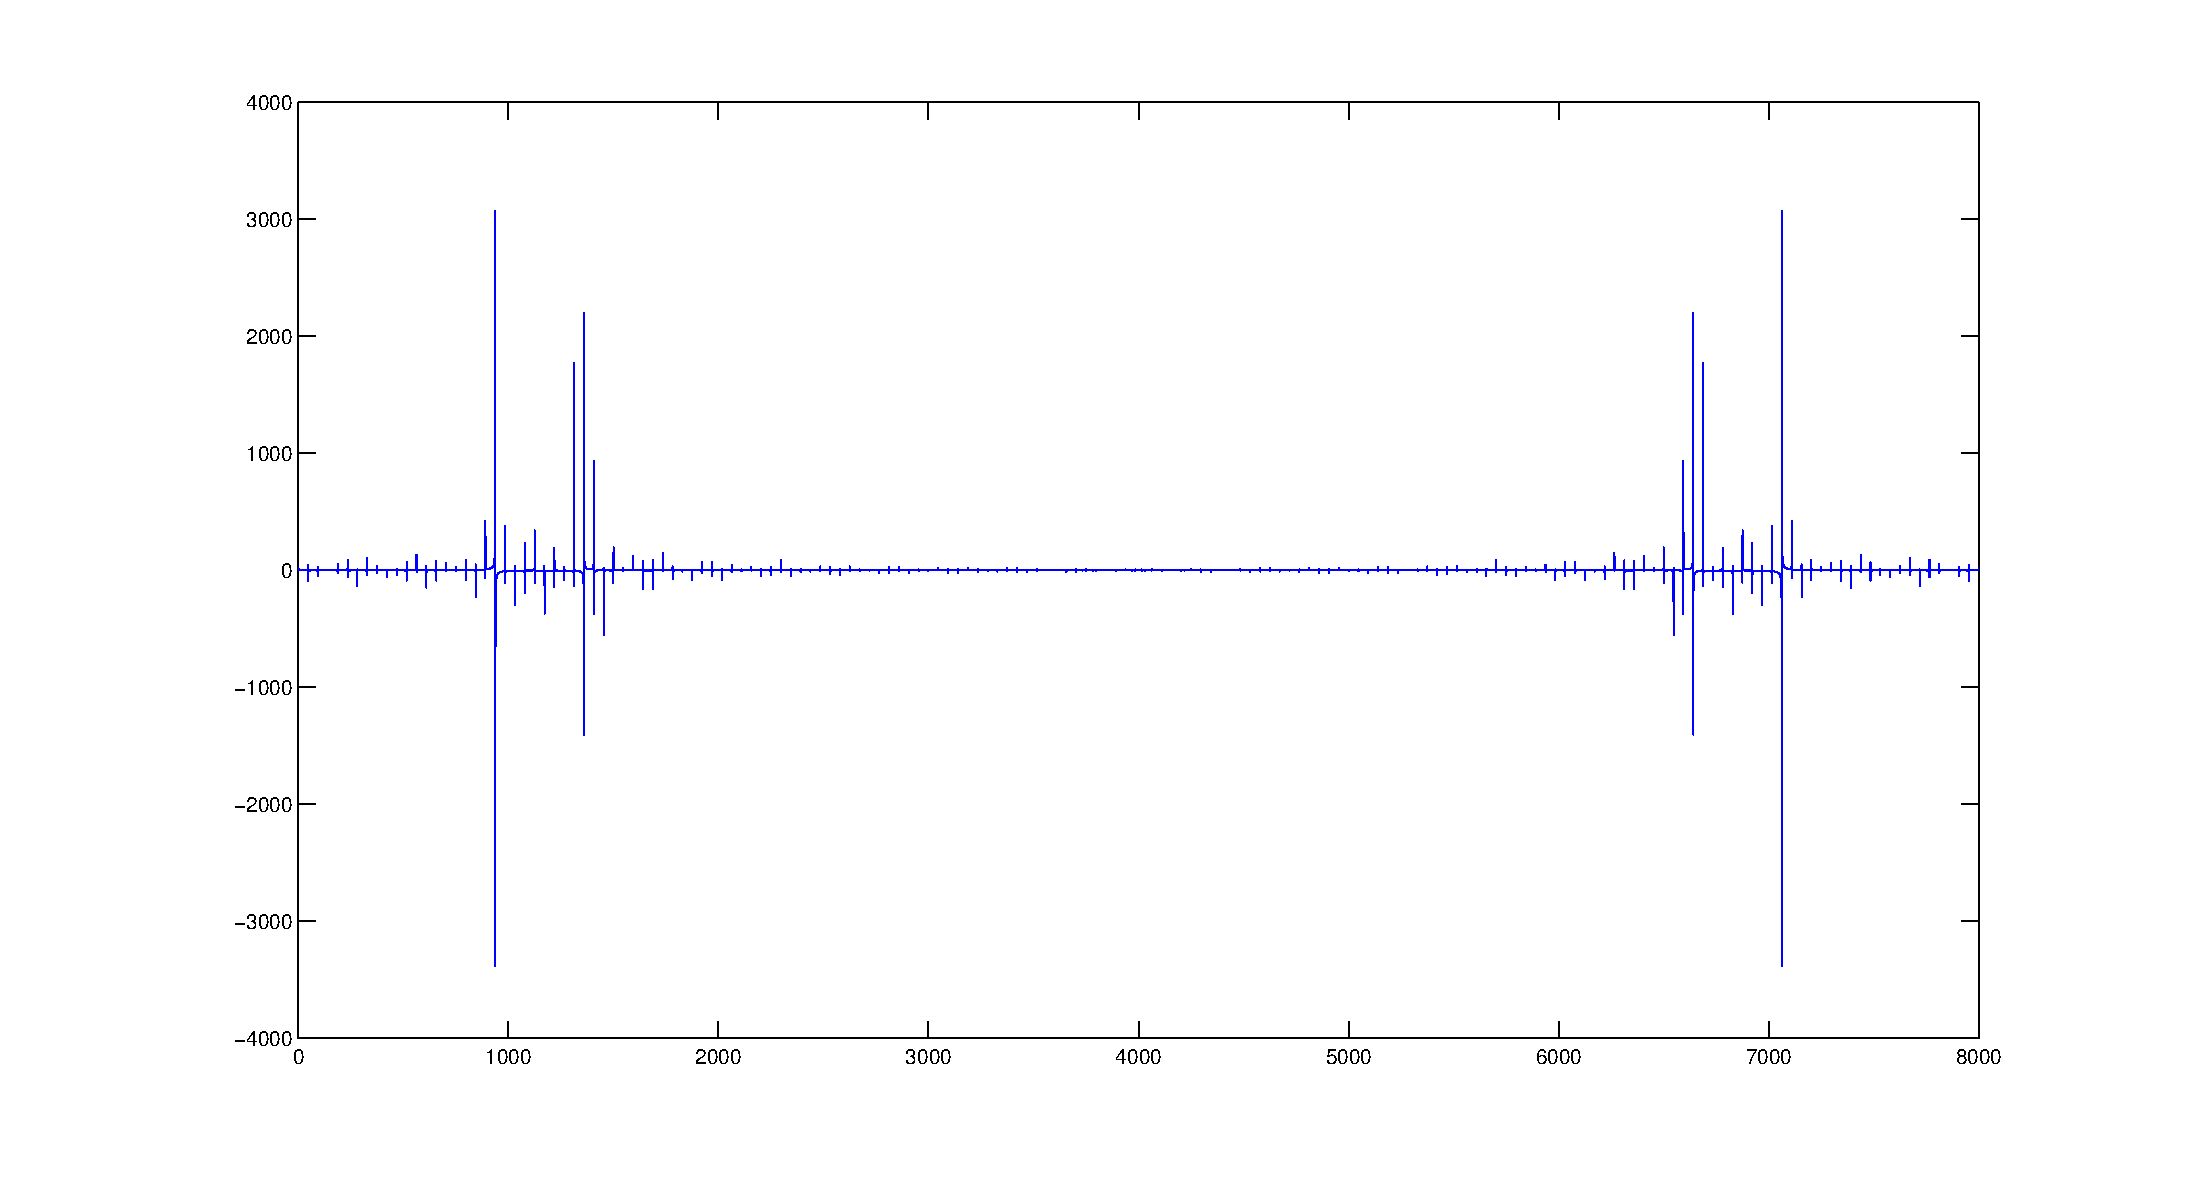
\includegraphics[width=0.45\textwidth]{2.eps}}
\caption{频域结果图,可以看见后面的图因为过采样的原因,频率的波形不连续}
\label{Fig.lable}
\end{figure}
作图的代码为:
\begin{lstlisting}
uiopen('/home/wtw/Desktop/test.wav',1)
a = data(:,1);
b = resample(a, 8000, 44100);
plot(b(1:100))
grid on;
c = fft(b); d = real(c)
plot([1:length(c)] * 8000 / length(c), d)
\end{lstlisting}
其中44100Hz是我们自带的录音软件的默认频率。
\subsection{DTMF信号的处理 \textcolor{red}{杨思怡部分}}
DTMF的信号产生严格按照我们实验指导书中的参考逻辑设计,具体代码如下:
\begin{lstlisting}
float goertzel(int numSamples, int TARGET_FREQUENCY,
        int SAMPLING_RATE, float* data) {

    int  k,i;
    float floatnumSamples;
    float omega, sine, cosine, coeff;
    float q0, q1, q2, result, real, imag;

    floatnumSamples = (float) numSamples;
    k = (int)(0.5 + ((floatnumSamples * TARGET_FREQUENCY)
                / SAMPLING_RATE));
    omega = (2.0 * M_PI * k) / floatnumSamples;

    sine = sin(omega);
    cosine = cos(omega);
    coeff = 2.0 * cosine;
    q0 = 0;
    q1 = 0;
    q2 = 0;

    for(i = 0; i < numSamples; i++) {
        q0 = coeff * q1 - q2 + data[i];
        q2 = q1;
        q1 = q0;
    }

    real = (q1 - q2 * cosine);
    imag = (q2 * sine);
    result = sqrtf(real * real + imag * imag);
    return result;
}
\end{lstlisting}
我们在proj2中提供了一个示例demo,在这个demo中,我们依次把结果输出来,得到的结果如下:
\begin{lstlisting}
Result of 697 is: 10.43
Result of 770 is: 118.65
Result of 852 is: 7.34
Result of 941 is: 11.86
Result of 1209 is: 10.12
Result of 1336 is: 120.45
Result of 1477 is: 10.34
Result of 1633 is: 9.12
The two freq is 1336 and 770!
\end{lstlisting}
这和我们的实际信号是符合,我们通过依次测试几个不同的信号,得到了对应的结果。
另外,和之前的示例文档保持一直,我们也采用了固态的系数来作为我们的demo。这个波形数据通过matlab转化成了在goetzel.h中定义的数组a。
\section{实验总结和感想}
\subsection{实验问题}
\subsubsection{问题一}
实验中遇到的最大的问题那就是我们网络学堂给的代码存在一定的问题。在上面的section中我们已经描述了这个问题。
当时我们花了超过3个小时的时间,和助教一起进行了很长时间的debug。非常感谢助教老师。\\
现在回顾,仔细想来其实是个很简单的错误,但是因为涉及到硬件,debug上有了很多麻烦。最后发现问题的关键是要使用标记变量,
把硬件的输出映射出来,在我们电脑上的IDE上进行查看。这样的话,我们的debug应该可以减少很多时间。\\
当时因为怀疑是硬件上的问题而不是软件上的问题,做了很多无用功。
\subsubsection{问题二}
因为我们的BF533板子并没有8000Hz的输出赫兹,我们需要进行一定的过采样。在这个地方,我们在理解数学上花了一些时间。
尤其是我们在使用autoBuffering的时候,多个频率,如果进行转换,是比较麻烦的。
autoBuffering中的FRAMESIZE,我们的输出采样频率\(f_s\),DTMF额定频率\(f_{DTMF}\),之间需要谨慎的转换。
具体的转换方式在上面已经说明了。根据我们的实验结果,我们应该尽量的减少autobuffering的大小。这是因为轮询程序本身的延时是非常大的。如果我们的FRAMESIZE过大,延迟效应会非常明显,产生混音,无法满足实时性条件。不过如果太小,中断的本身时间开销又会带来过大的消耗。
\subsubsection{问题三}
在matlab上进行验证的时候,我们需要调整采样率。这是因为我们的附件中的录音程序的额定频率是44.1kHz,一般来说为了验证我们的输出信号,我们需要resample到8000Hz,取每800个采样点的中间400个采样点进行分析。同时需要验证头尾200采样点是否保持了静音。
\subsection{实验感想}
最后的大作业是一个软硬件协同的软件,个人觉得难度比较大,同时了锻炼了很多协作的能力。整个DSP课程非常合理,从无到有,深入浅出。从最开始最简单的IDE平台的使用,到汇编C语言混合编程,到最后的硬件实现,整个课程的体系非常明晰。感觉学到了非常多的东西,非常感谢老师。\\
五次实验和最后的大作业的内容分配十分合理,让我们循序渐进的认识到DSP开发板的全面强大的功能,在音频、图像、视频信号处理均能完成。延续之前几次的重点内容,我们选择了在大作业中继续对音频信号进行处理。从信号的生成和处理两方面都由自己完成,让我们更加深刻的把握和理解了DSP硬件在处理信号中的重要性。\\
然而同时我们也希望老师把课程的难度进行一定的调整。例如第二次上机实验的难度比较大,同学们往往不能在一个下午的五个小时之内完成,晚上来做实验的同学大多都没能在时间内顺利完成,必须要另外单开一次实验。\\
非常感谢老师和助教老师!
\end{CJK}
\end{document}
\begin{lstlisting}
